\documentclass[openany]{book}
\title{Microeconomía}
\author{David Gabriel Corzo Mcmath}
\date{2020-Jan-06 11:36:01}
%%%%%%%%%%%%%%%%%%%%%%%%%%%%%%%%%%%%%%%%%%%%%%%%%%%%%%%%%%%%%%%%%%%%%%%%%%%%%%%%%%%%%%%%%%%%%%%%%%%%%%

\usepackage[margin = 0.8in]{geometry}
\usepackage{graphicx}
\usepackage{fontenc}
\usepackage{pdfpages}
\usepackage[spanish]{babel}
\usepackage{amsmath} % [intlimits]
\usepackage{amssymb}
\usepackage{amsthm}
\usepackage{mathtools}
\usepackage[utf8]{inputenc}
\usepackage{enumitem}
\usepackage{pdfpages}
\usepackage{blindtext}
\usepackage{fancyhdr}
\usepackage{tikz}
\usepackage{hyperref}
\usepackage{longtable}
\usepackage{generalsnips}
\usepackage{calculussnips}
\usepackage{cancel}

\thispagestyle{empty}
\pagestyle{plain}

\pdfsettings
%%%%%%%%%%%%%%%%%%%%%%%%%%%%%%%%%%%%%%%%%%%%%%%%%%%%%%%%%%%%%%%%%%%%%%%%%%%%%%%%%%%%%%%%%%%%%%%%%%%%%%%%%%%%%%%%%%%%%%%%%%%%%%%%%%%%%%%%%%%%%%%
\begin{document}
\maketitle
\tableofcontents

\chapter{Elasticidad}
\includepdf[pages=-,pagecommand={\thispagestyle{plain}}]{./Clases/Elasticidad.pdf}
\input{Clases/ElasticidaYTeoriaDeLaEmpresa.tex}

\chapter{Control de precios}
\includepdf[pages=-,pagecommand={\thispagestyle{plain}}]{./Clases/Control_De_PreciosYElasticidad.pdf}
\includepdf[pages=-,pagecommand={\thispagestyle{plain}}]{./Clases/Comercio_Internacional.pdf}
\includepdf[pages=-,pagecommand={\thispagestyle{plain}}]{./Clases/ExcedenteProductoryConsumidor.pdf}

\chapter{Teoría de la empresa y del productor}
\input{Clases/TeoriaDeLaEmpresa.tex}
\section{Principios}
\begin{enumerate}
    \item Las personas enfrentan disyuntivas / las personas siempre están tomando decisiones.
    \item Las personas piensan en términos marginales.
    \item Las personas buscan maximizar sus beneficios.
\end{enumerate}

%%%%%%%%%%%%%%%%%%%%%%%%%%%%%%%%%%%%%%%%%%%%%%%%%%%%%%%%%%%%%%%%%%%%%%%%%%%%%%%%%%%%%%%%%%%%%%%%

\section{Recordar}
\begin{itemize}
    \item \emph{\textbf{Recordar lo siguiente: }Los modelos no representan en su plenitud la realidad.}
    \item Es economía neoclásica, vivimos en un mundo de escasez.
\end{itemize}


\section{Tasa marginal de sustitución}
\begin{itemize}
    \item \[
        TMS = \frac{MU_x}{MU_y} 
      \]
    
    \item TMS: Puede ser expresada en términos de utilidades marginales.
    \item Derivadas parciales: ejemplo, derivada parcial con respecto a x es :     
        \begin{align*}
            f(x) = 3x y \\ 
            % f'(x) = 3\cancel{x}y \\
            \therefore f'(x) = 3y \\ 
        \end{align*}
\end{itemize}

%%%%%%%%%%%%%%%%%%%%%%%%%%%%%%%%%%%%%%%%%%%%%%%%%%%%%%%%%%%%%%%%%%%%%%%%%%%%%%%%%%%%%%%%%%%%%%%%

\section{Tasa de transformación}
\begin{itemize}
    \item La pendiente de la restricción presupuestaria.
    \item TMT:
        \begin{align*}
            TMT = -\frac{P_x}{P_y} \\ 
        \end{align*}
\end{itemize}


%%%%%%%%%%%%%%%%%%%%%%%%%%%%%%%%%%%%%%%%%%%%%%%%%%%%%%%%%%%%%%%%%%%%%%%%%%%%%%%%%%%%%%%%%%%%%%%%

\section{Efectos por el cambio de precio}
\begin{itemize}
    \item Todas las combinaciones óptimos de las curvas de indiferencia forma la \emph{curva de demanda}.
    \item Curva de precio consumo: la línea que traza las combinaciones óptimas como respuesta a un cambio de precio, manteniendo el ingrso constante. 
    \item La unión de las combinciones óptimas de las curvas de indiferencia respecto de los cabios de precio.
\end{itemize}

%%%%%%%%%%%%%%%%%%%%%%%%%%%%%%%%%%%%%%%%%%%%%%%%%%%%%%%%%%%%%%%%%%%%%%%%%%%%%%%%%%%%%%%%%%%%%%%%

\section{Efectos por el cambio en el ingreso}
\begin{itemize}
    \item Curva de ingreso consumo: es la unión de los puntos óptimos respecto a los cambios en nuestros ingresos.
\end{itemize}


%%%%%%%%%%%%%%%%%%%%%%%%%%%%%%%%%%%%%%%%%%%%%%%%%%%%%%%%%%%%%%%%%%%%%%%%%%%%%%%%%%%%%%%%%%%%%%%%

\section{Curva de ingreso consumo}
\begin{itemize}
    \item Tomar en cuenta:
        \begin{enumerate}
            \item Bien normal: sube el ingreso, sube la demanda de un bien.
            \item Bien inferior: sube el ingreso, dejo de demandar ese bien.
        \end{enumerate}
    
    \item Considerar lo siguiente: puede ser que cuando aumente el ingreso se mantenga constante con la alternativa de \textbf{ahorrar}, \emph{\textbf{Interesante:} Ahorrar se considera como un bien normal}.
    \item Un bien no siempre va a ser inferior o normal.
    \item La unión de los puntos óptimos de las curvas de indiferencia, la curva de ingreso consumo es equivalente a decir la \emph{curva de Engel}.
\end{itemize}

%%%%%%%%%%%%%%%%%%%%%%%%%%%%%%%%%%%%%%%%%%%%%%%%%%%%%%%%%%%%%%%%%%%%%%%%%%%%%%%%%%%%%%%%%%%%%%%%

\section{Fórmulas}
\begin{itemize}
    \item Restricción presupuestaria:
        \[
          Y = Q_vP_v \times Q_qP_q
        \]
\end{itemize}








\chapter{Empresa en un mercado perfectamente competitivo}
\input{Clases/Repaso.tex}


\chapter{temp}
\section{Empresa vs. Mercado}
\begin{figure}
    \centering
    % \includegraphics[width=8cm]{./Clases/figs/}
\end{figure}

\subsection{Procedimiento}
\begin{itemize}
    \item Inciso:
        \begin{center}
            \begin{figure}[!htb]
                \centering
                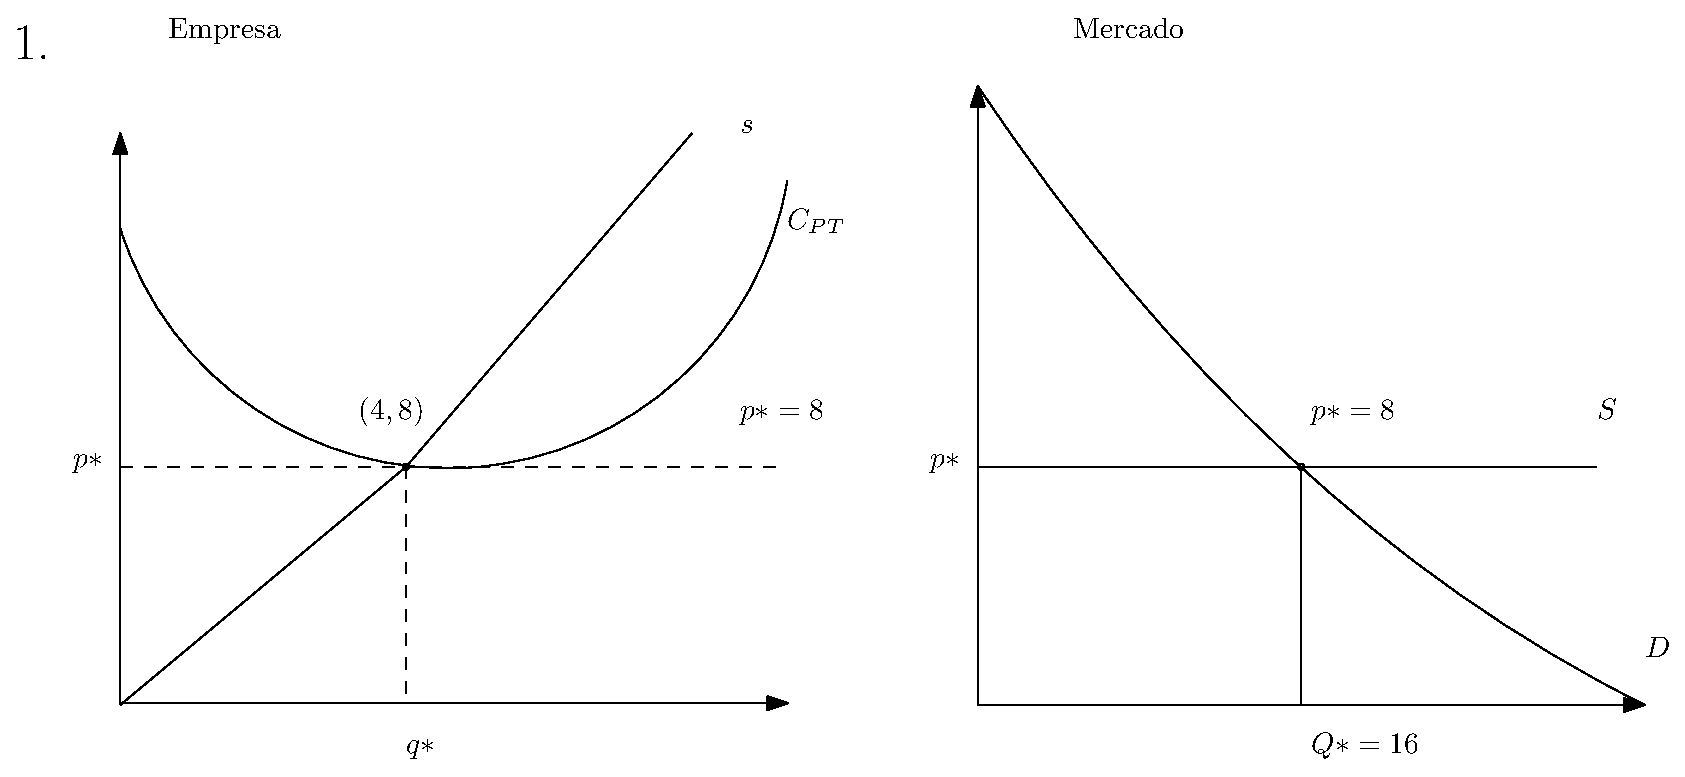
\includegraphics[width=18cm]{./Clases/figs/01.eps}
            \end{figure}
        \end{center}
        \begin{itemize}                
        \item Debemos sacar el $p*$ \& $q*$ 
        \end{itemize}
        \begin{center}
           \begin{align*}
               C_T &= 16 + q^2 \\ 
               Q &= 24 - p \\ 
               \text{ Min.  }\; C_{PT}: \\ 
                    \frac{C_T}{q} &= \frac{16+q^2}{q} \\ 
                    \text{ Costo promedio Total }: \qq C_{PT} &= \frac{16}{q} + q \\ 
                    \text{ Derivamos }: \qq   
                        \dervpar{C_{PT}}{q} &= -16q^{-2} + 1 \\  
                        \text{ Igualar a 0 }: \qq  -16q^{-2} + 1 = 0 \qimplies q* = 4 \\ 
                C_{PT}(q*=4) &= \frac{16+(4)^2}{4} = 8 \\  
                \therefore \qq \text{ El precio \&  la cantidad es:  }\; p*&=8, q*=4, Q*=16 \\ 
           \end{align*}
        \end{center}
    
    \item Inciso: 
        \begin{itemize}
            \item Dadas las siguentes funciones: 
                \begin{center}
                    \begin{figure}[!htb]
                        \centering
                        \includegraphics[width=18cm]{./Clases/figs/02.eps}
                    \end{figure}
                \end{center}
                \begin{center}
                   \begin{align*}
                       C_{T} &= 10q^2+10 \qq \qq Q = 1,000-p \\ 
                   \end{align*}
                   \begin{itemize}
                       \item Sacar: $q*$, $Q*$, $p*$ y el número de empresas.  
                   \end{itemize}
                   \begin{align*}
                       C_{TP} &= \frac{10q^2+10}{q} = 10q +\frac{10}{q} \\
                       \dervpar{C_{PT}}{q} &= 10 - 10q^{-2} \qimplies q* = 1 \\  
                       C_{TP}(q*=1) &= 10(1)^1 + \frac{10}{1} = 20 \\ 
                       \therefore \qq C_{TP}&=20 \; \text{ ó }\; p*=20, q*=1 \\   
                   \end{align*}
                \end{center}
        \end{itemize}
\end{itemize}


\chapter{1. Cálculo del excedente del productor y consumidor, \\2. Precios máximos y mínimos, \\ 3. Impuestos. \\ Todo con integrales}
\section{Excedente del productos y del consumidor}
\begin{itemize}
    \item Asumir que estamos en equilibrio.
    \item Excedente del consumidor:
        \[
          C_S = \int_{0}^{Q*}\left[P(Q^D)-P*\right]dQ^D
        \]
    
    \item Excedente del productor:
        \[
          P_S = \int_{0}^{Q*}\left[ P*-P(Q^s) \right] dQ^s
        \]
    
    \item Excedente del consumidor y productor:
        \begin{figure}[!htb]
            \centering
            \includegraphics{Clases/figs/03}
        \end{figure}
    
    \item Precio máximo: El precio máximo está por debajo de equilibrio: $\displaystyle P_C < P*$ $\displaystyle Q_C$ es la cantidad vendida al precio máximo y $\displaystyle P_C$ es el precio máximo. 
        \[
          C_{S_C} = \int_{0}^{Q_c}\sqb{P\p{Q^D} -P_C} dQ^{\square}
        \]
        \[
          P_{S_C} = \int_{0}^{Q_C} \sqb{P_C-P\p{Q^S} } dQ^{\square}
        \]
        \begin{figure}[!htb]
            \centering
            \includegraphics{Clases/figs/05}
        \end{figure}
    
    \item Precio mínimo: El precio mínimo estpa porarriba del precio de equilibrio: $\displaystyle P_f > P*$ y $\displaystyle Q_f$ es la cantidad demandada con el precio mínimo. $\displaystyle P_f$ es el precio mínimo.  
        \begin{figure}[!htb]
            \centering
            \includegraphics[]{Clases/figs/04} 
        \end{figure}
        
    \item Impuestos: 
        \begin{figure}[!htb]
            \centering
            \includegraphics[]{Clases/figs/06} 
        \end{figure}
\end{itemize}


%----------------------------------------------------------------------------------------
\subsection{Ejercicio}
\begin{itemize}
    \item Demanda de Widgets: $\displaystyle D(q) = 200-q^2$ Oferta: $\displaystyle S(q) = q^2+38$, Encontrar CS y PS:  
        \begin{center}
           \begin{align*}
               q* = 9 \qq & \qq p*=119 \\ 
               C_S &= \int_{0}^{9}\p{200-q^2-119} dq \\ 
                &= 200q-\frac{q^3}{3} -119q \qq \evaluate{0}{9} \\ 
                & = \text{ \$ }486 \\ 
           \end{align*}
        \end{center}
\end{itemize}



\end{document}
